\section{Results}\label{sec:results}
%Mention something about the distribution of the data? And choice of baseline model.
% ==================================================================
%
% Jo writes here
% Decision tree 
% - performance
\subsection{Decision tree and AdaBoost (classical features)}
We started by performing a grid search for the decision tree, using the metadata from the PlanktoScope images. The parameters tested and optimal parameters can be found in Table \ref{tab:params_tree}. Since max depth was set, the models were trained using a pre-pruning method. To evaluate the model performance we used a 10-fold cross-validation and the accuracy score as evaluation metric.
\begin{table}[h]
    \centering
    \begin{tabular}{ccc}
        \hline
        \verb|max_depth| \, & \verb|min_samples_split| \, & \verb|criterion| \\
        \hline 
        $5$ & $5$ & \verb|gini|$^*$ \\
        $10^*$ & $10$ & \verb|entropy| \\
        $15$ & $15$ & \\
        $20$ & $20^*$ & \\
        \hline
    \end{tabular}
    \caption{Parameters tested when performing a grid search for the decision tree method, where * marks the best results. The models were trained and tested on the metadata from the PlanktoScope}
    \label{tab:params_tree}
\end{table}

The optimal parameters show that the best criterion for splitting is gini, with a max depth of $10$ and a minimum of $20$ samples per split. The accuracy on both train and test data was approx. $78\%$, indicating a well fit model with a balance between complexity and fit. 
We continued with the optimal model, and plotted a confusion matrix to investigate the predicted labels. The result is shown in Figure \ref{fig:cm_tree_metadata}, where the label names can be found in Table \ref{tab:target_names} in Appendix \ref{ap:decision_adaboost}.
% Performance using optimal parameters
\begin{figure}
    \centering
    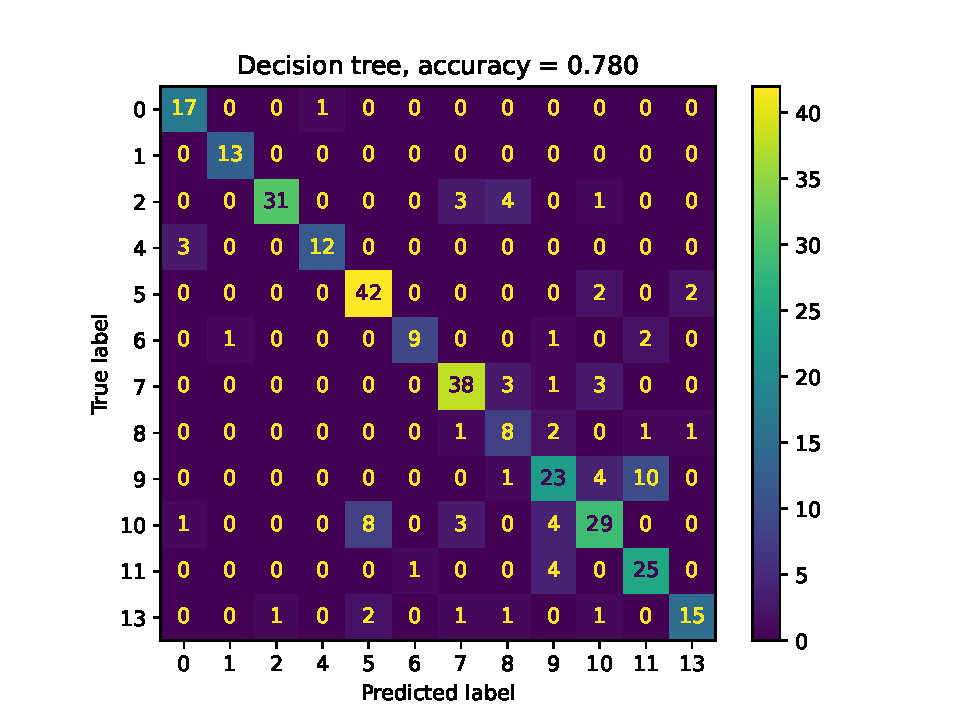
\includegraphics[width=\linewidth]{latex/figures/cm_tree_planktoscope_metadata.pdf}
    \caption{Caption}
    \label{fig:cm_tree_metadata}
\end{figure}
The model has difficulties predicting the correct label for 9:Tripos furca, and predicts either 10:Tripos fusus or 11:Tripos muelleri. The most important features in predicting the target species were \verb|object_equivalent_diameter| and \verb|object_perimareaexc|, with values of approx. $0.18$ and $0.17$, respectively. The feature importance of the remaining features can be found in Appendix \ref{ap:decision_adaboost}, Table \ref{tab:dt_ft_imp}. One interesting thing to mention is that the object size in it self was not an important feature, however, the information can likely be explained by other features.
% Adaboost 
% - grid search results
% - performance
To explore the potential of performance increase, we continued with the AdaBoost method using decision tree as the weak classifier. As for the decision tree, we performed a grid search using the parameters found in Table \ref{tab:params_adaboost}. 
\begin{table}[h]
    \centering
    \begin{tabular}{ccc}
        \hline
        \verb|max_depth| \, & \verb|n_estimators| \, & \verb|learning_rate| \\
        \hline 
        $1$ & $100$ & $0.001$ \\
        $2^*$ & $500$ & $0.01$ \\
         & $1000^*$ & $0.1$ \\
         & & $1.0^*$ \\
        \hline
    \end{tabular}
    \caption{Parameters tested when performing a grid search for the AdaBoost method. $*$ indicate the best parameters for the models trained and tested on the metadata from the PlanktoScope.}
    \label{tab:params_adaboost}
\end{table}
We continued with entropy as criterion for splitting, and used the same data as in previous grid search for the decision tree. However, the data was split into three set, to measure the error when increasing number of weak classifiers on a separate validation set. In Figure \ref{fig:cm_adaboost_metadata}.
\begin{figure}
    \centering
    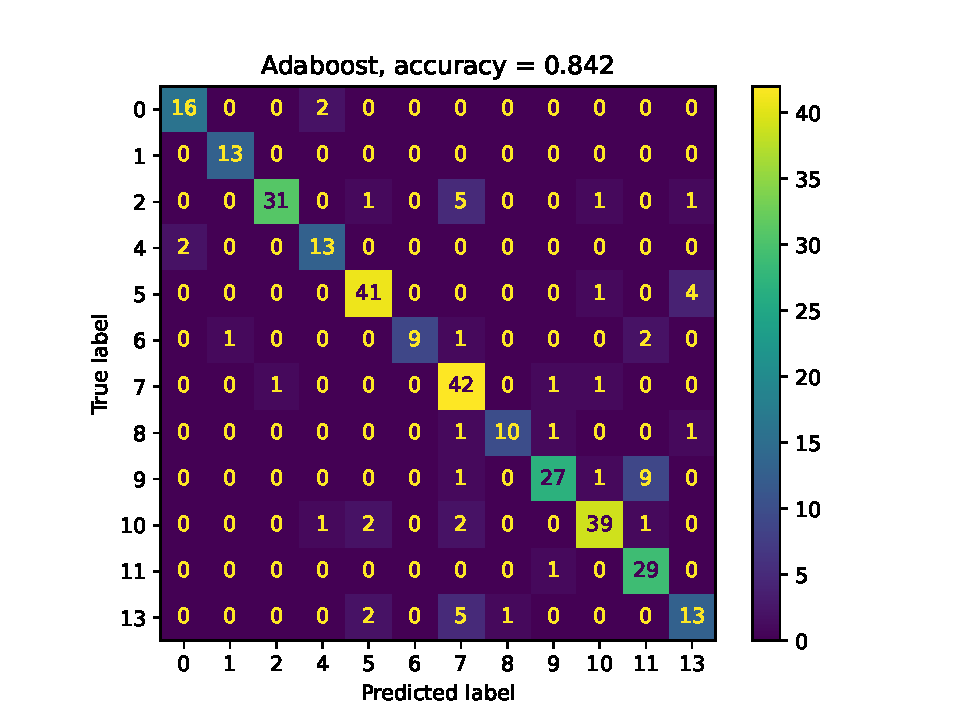
\includegraphics[width=\linewidth]{latex/figures/cm_adaboost_planktoscope_metadata.pdf}
    \caption{Caption}
    \label{fig:cm_adaboost_metadata}
\end{figure}
Again, the model wrongly predict 9:Tripos furca. However, most of the predictions are 11:Tripos muelleri, which is an improvement from the decision tree. All features show some importance for AdaBoost, in contrast to the decision tree. Since the result from each weak classifier is weighted when making a final prediction, which likely result in all the features being candidates for at leat one weak classifier. However, the most important feature for prediction was \verb|object_perimareaexc|, with a feature importance value of approx. $0.1612$. This was also one of the most important features in predicting with the decision tree model, and it has a similar value for both models. The remaining feature importances for AdaBoost can be found in Appendix \ref{ap:decision_adaboost}, Table \ref{tab:adaboost_ft_imp}. 

The AdaBoost model show a significant increase in performance when compared to the decision tree, with a train and test accuracy of approx. $85.7\%$ and $84.2\%$, respectively. We investigated the decrease in error as number of trees (estimators) increase, the result is shown in Figure \ref{fig:be_adaboost_metadata}. 
\begin{figure}
    \centering
    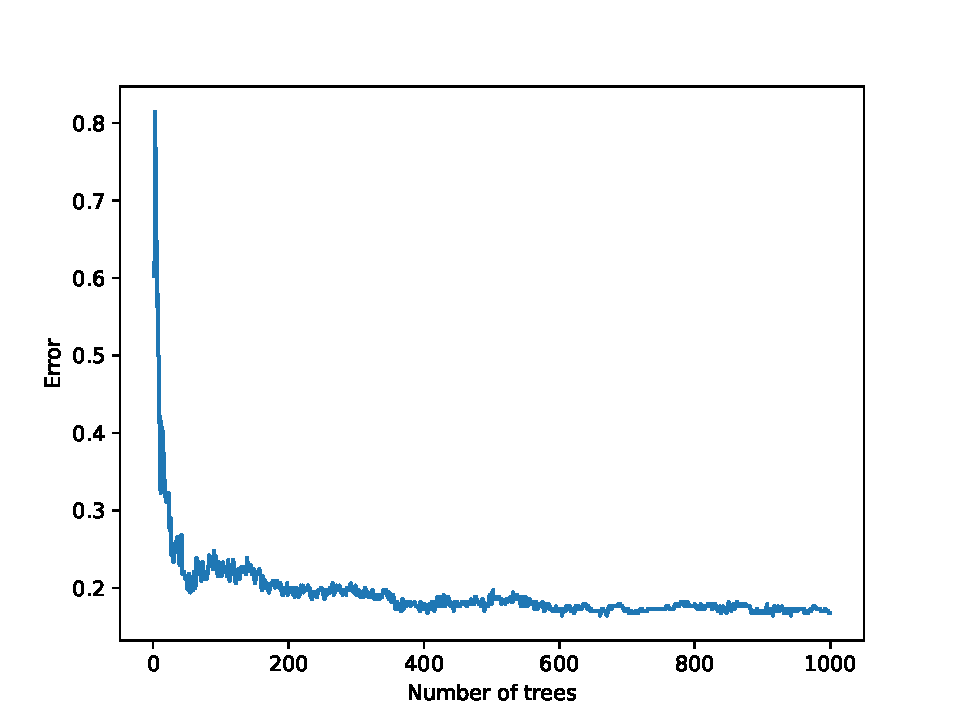
\includegraphics[width=\linewidth]{latex/figures/be_adaboost_planktoscope_metadata.pdf}
    \caption{Caption}
    \label{fig:be_adaboost_metadata}
\end{figure}
The error decrease is most significant for the first $50$ estimators. After $400$ estimators there is no significant decrease in error. The grid search result indicated that a higher number of estimators might give better results, since the optimal value was the largest tested. However, the decrease in error does not necessarily justify the increase in computational cost.
%Results for dino features after dino results :)
% ==================================================================

\subsection{Convolutional Neural Networks}

We used the PlanktoScope data to select the best CNN for predicting on plankton images. Normalizing each layer of the image, according to REF, made the model reach maximum accuracy faster (Figure \ref{fig:epochs}). Since the normalized data reached maximum validataion accuracy after around 20 epochs, we chose to use 30 epochs when grid-searching for parameters, as a tradeoff between computation time and model convergence.

\begin{figure}
    \centering
    \begin{subfigure}{1\linewidth}
        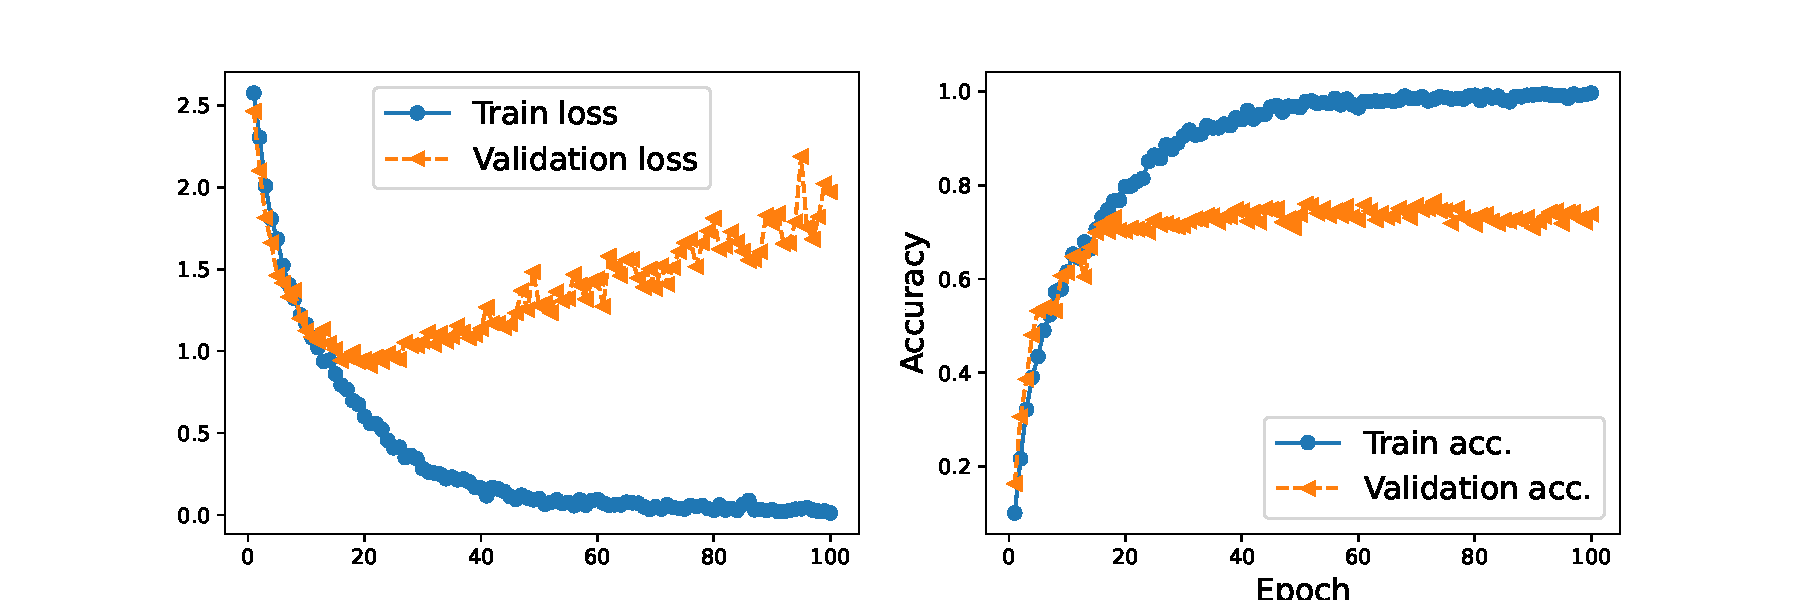
\includegraphics[width=\linewidth]{examples/tests_even/figs/CNN-test-epochs100-64.pdf}
        \caption{Normalized input}
        \label{fig:epochs1}
    \end{subfigure}
    \begin{subfigure}{1\linewidth}
        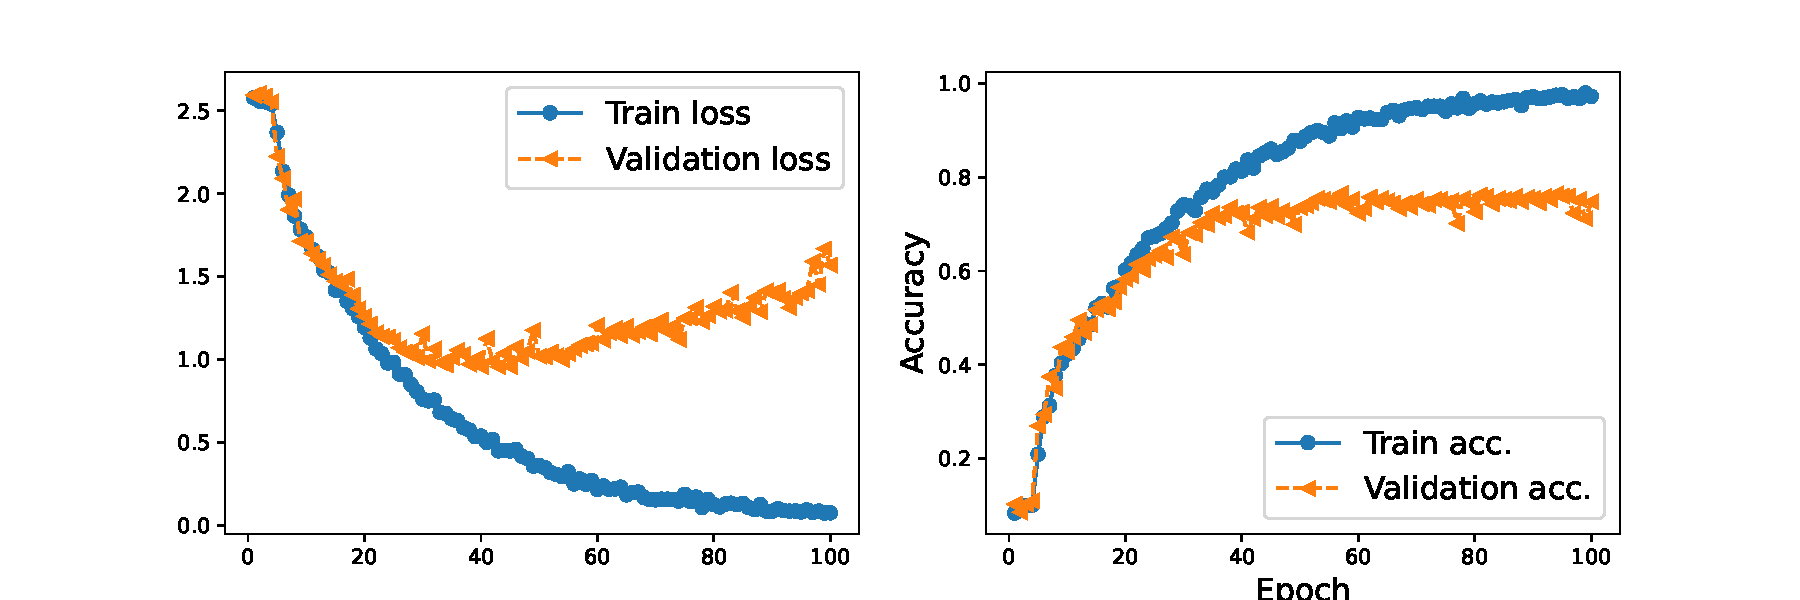
\includegraphics[width=\linewidth]{examples/tests_even/figs/CNN-test-epochs100-64notnorm.pdf}
        \caption{Non-normalized input}
        \label{fig:epochs2}
    \end{subfigure}
    \caption{The convergence by number of epochs for normalized (a) and non-normalized (b) input data. For the normalized data, the three layers of the image (r,g,b) were first minmax scaled, and then normalized with respective means 0.485, 0.456 and 0.406 and standard deviations 0.229, 0.224 and 0.225. The non-normalized data was only minmax scaled. The normalized input reached the maximum accuracy much faster than the non-normalized.}
    \label{fig:epochs}
\end{figure}


First, we tested three different CNNs, with 1, 2 and 3 convolutional layers, respectively. The CNN with 3 layers outperformed those with 1 and 2 (Figure \ref{fig:gridsearch-nconv}), and we chose 3 layers in our network for all subsequent analyses. The network performed best with a learning rate of $1.6 \cdot 10^{-4}$, and L2 regularization with $\lambda = 10^{-3}$ (Figure \ref{fig:gridsearch-planktoscope}). The best model with L2 regularization was also slightly better than that without (accuracy 0.74 vs 0.73, without regularization shown in Figure \ref{fig:gridsearch-nconv}). The final architecture of the CNN is shown in Figure \ref{fig:conv-arch}.






\begin{figure}
    \centering
    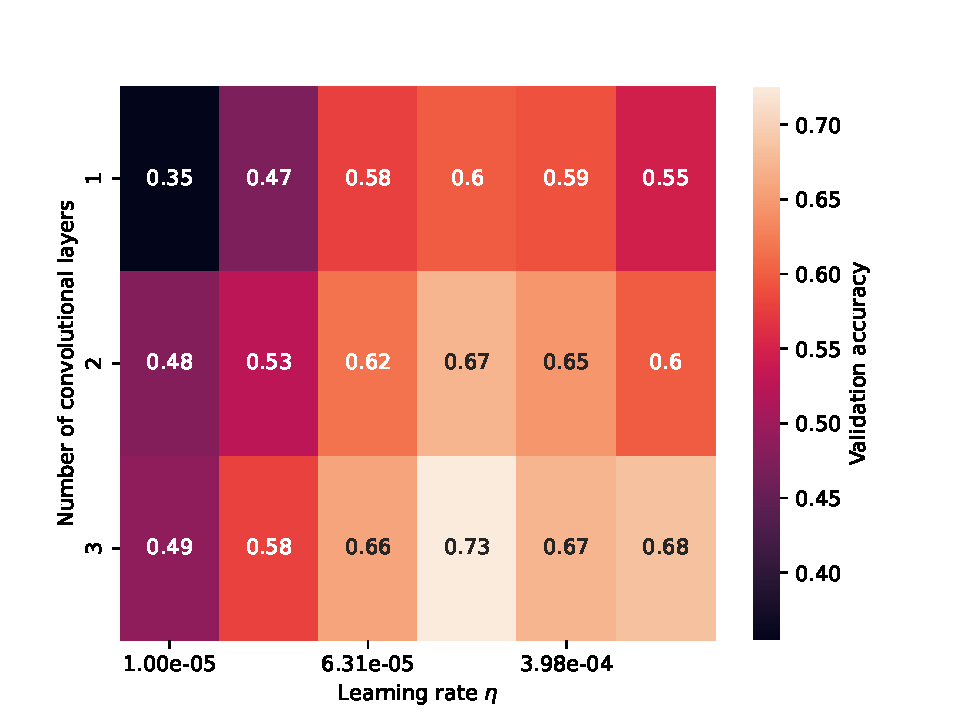
\includegraphics[width=\linewidth]{examples/tests_even/figs/gridsearch-nconv-128-2024-12-12_1108.pdf}
    \caption{Grid search finding the optimal number of convolutional layers (CONV) of a convolutional neural network on the PlanktoScope data. The network with the best accuracy on the validation set used 3 CONV and had a learning rate $\gamma = 1.6 \cdot 10^{-4}$, and reached an accuracy of 0.73 after 30 epochs.}
    \label{fig:gridsearch-nconv}
\end{figure}

\begin{figure}
    \centering
    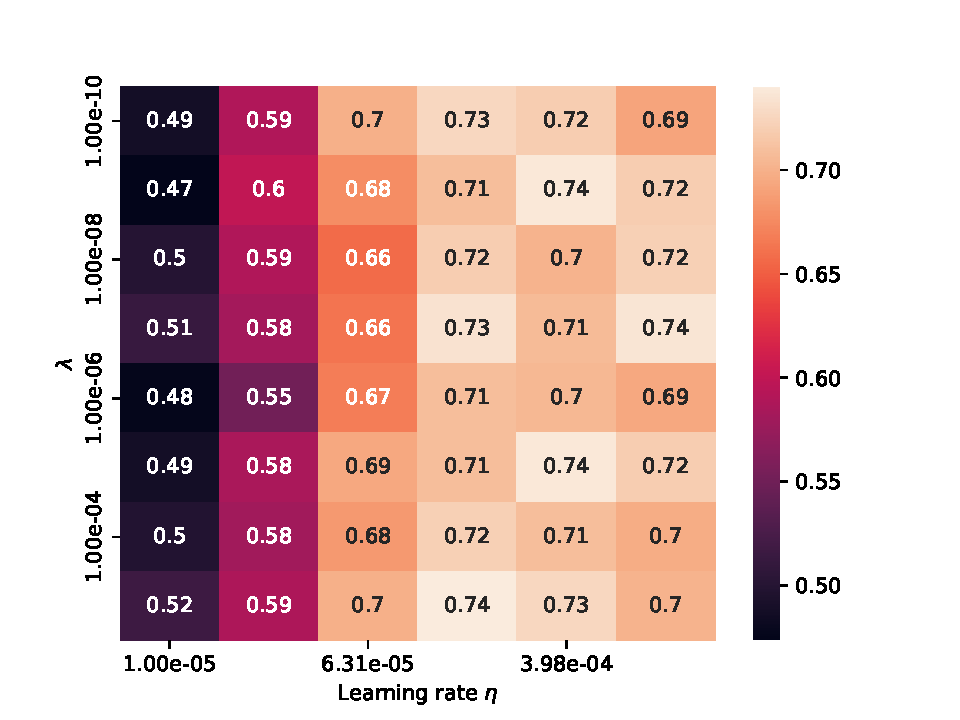
\includegraphics[width=\linewidth]{examples/tests_even/figs/gridsearch-128-2024-12-06_1241.pdf}
    \caption{Grid search of learning rate $\gamma$ and the regularization parameter $\lambda$ on the PlanktoScope data. The best accuracy on the training data was 0.74, with $\gamma = 1.6 \cdot 10^{-4}$ and $\lambda=10^{-3}$. Note that the best learning rate stayed the same from the grid in figure \ref{fig:gridsearch-nconv} The best model chosen here was used for the predictions in figure \ref{fig:confusion-planktoscope}}
    \label{fig:gridsearch-planktoscope}
\end{figure}

\begin{figure}
    \centering
    \includegraphics[width=\linewidth]{latex/figures/convnet\_architecture.png}
    \caption{The final architecture of the convolutional neural network used to analyze the PlanktoScope data. The final model was trained with learning rate $\gamma=1.6 \cdot 10^{-4}$ regularization parameter $\lambda = 10^{-3}$}
    \label{fig:conv-arch}
\end{figure}

The final model had a accuracy of 0.72 on the test data, and generally taxa were predicted to their true label (Figure \ref{fig:confusion-planktoscope}). Like for the decision tree and AdaBoost, the CNN misclassified the different species of \textit{Tripos}, with the most common mistake being to label \textit{Tripos muelleri} as \textit{Tripos furca}. The CNN failed in classifying \textit{Oithona}, which was the speciest with the lowest sample size in our data. In addition it made some Several of the other images that were misclassified had multiple species or detritus present, or were out of focus (Figure \ref{fig:cnn-wrong-ps})

\begin{figure}
    \centering
    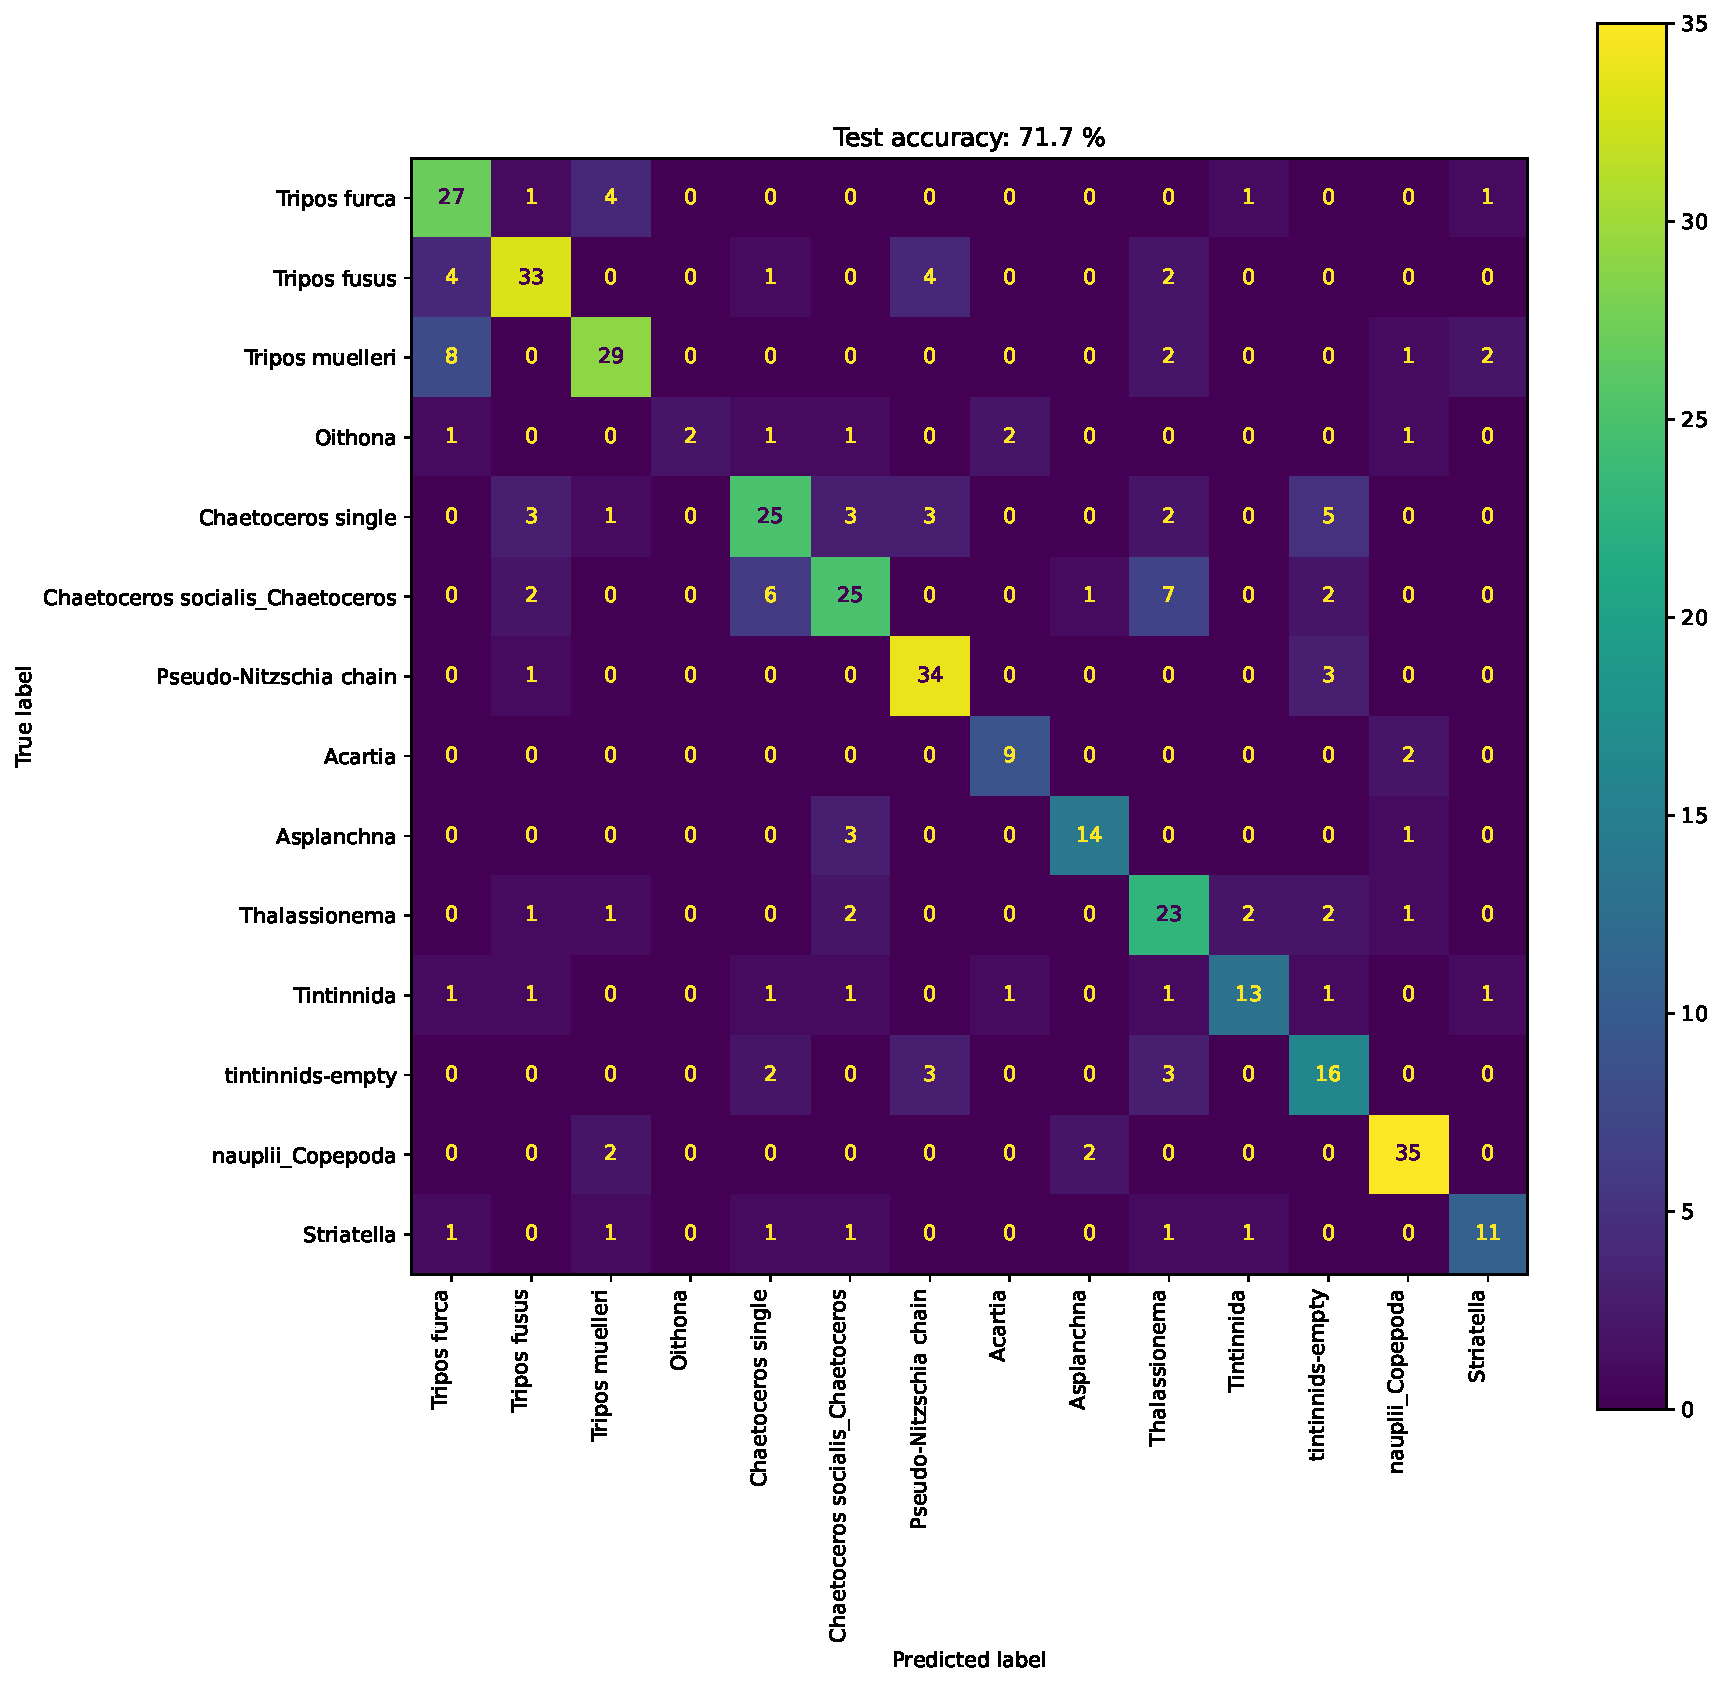
\includegraphics[width=\linewidth]{examples/tests_even/figs/confusion-matrix-2024-12-06_1241.pdf}
    \caption{Confusion matrix for the best model from the grid search (figure \ref{fig:gridsearch-planktoscope}) run on the test data (20\% of the full data set). The category where the model performed the worst was for \textit{Oithona}, where only 2 of 8 predictions were correct. This was, however, also the category with the fewest images, with 59 versus 200 in most of the other.}
    \label{fig:confusion-planktoscope}
\end{figure}


% \begin{table}
%     \centering
%     \begin{tabular}{cllccl}
%          CONV layer&    Layers in&Layers out&Parameters& Activation &Pooling\\
%          CONV1&    3 (128x128 pixels)&32&$s=1, p=2$, $\text{kernel\_size}=5$&  ReLU&Max\\
%          CONV2&    32&64&$s=1, p=2$, $\text{kernel\_size}=5$&  ReLU&Max\\
%          CONV3&    64&128&$s=1, p=2$, $\text{kernel\_size}=5$&  ReLU&Max\\
%          FC layer&    Nodes in&Nodes out&&  &\\
%          FC1&    &1024&&  ReLU&\\
%          Dropout&    &&$p=0.5$&  &\\
%          FC2&    1024&400&&  ReLU&\\
%          Dropout&    &&$p=0.5$&  &\\
%          FC3&    400&Num categories&&  softmax&\\
%     \end{tabular}
%     \caption{Final architechture of the convolutional neural network}
%     \label{tab:my_label}
% \end{table}


% ==================================================================
%
% EB writes here
%
\subsection{DINOv2 ViT}
We extracted 384 features for each of the 2061 images [camera type here], inserted them into a design matrix with rows containing a numerical feature and columns containing the image they originated from. The resulting 2961 x 384 matrix was then standardized and reduced with either PCA with 70 principal components, or UMAP with 2 embeddings. 

We present the first two components of the PCA plotted against each other in Figure \ref{fig:pca0pca1}, and the embeddings from UMAP in Figure \ref{fig:umap}. Both figures have labeled species data points, but this labels have not been provided for the DINO ViT model and are provided afterwards to see whether the feature representations we've retrieved can be considered good representations.

After analyzing the cumulative variance for each component (Appendix, Figure \ref{fig:cumsumpca}), we saw that including 70 components accounted for just above 85\% of the variance in the design matrix, and the first two components only account for around 26\%. This means that we cannot assume the PC representations to relay significant relationships in our data. 

In Figure \ref{fig:umap} we see clear clusters. We already know that the input images belonged to 14 categories, and yet we count 11 distinct cluster which is also confirmed by the silhouette score for each of the 2-20 KMeans clusters we tested (Appendix, Figure \ref{fig:kmean_sil}). We suspect that the species that have similar feature embeddings might also have some morphological similarities, which is confirmed by looking into some example photos in Figure \ref{fig:pseudo+empty}. 

\begin{figure}[H]
    \centering
    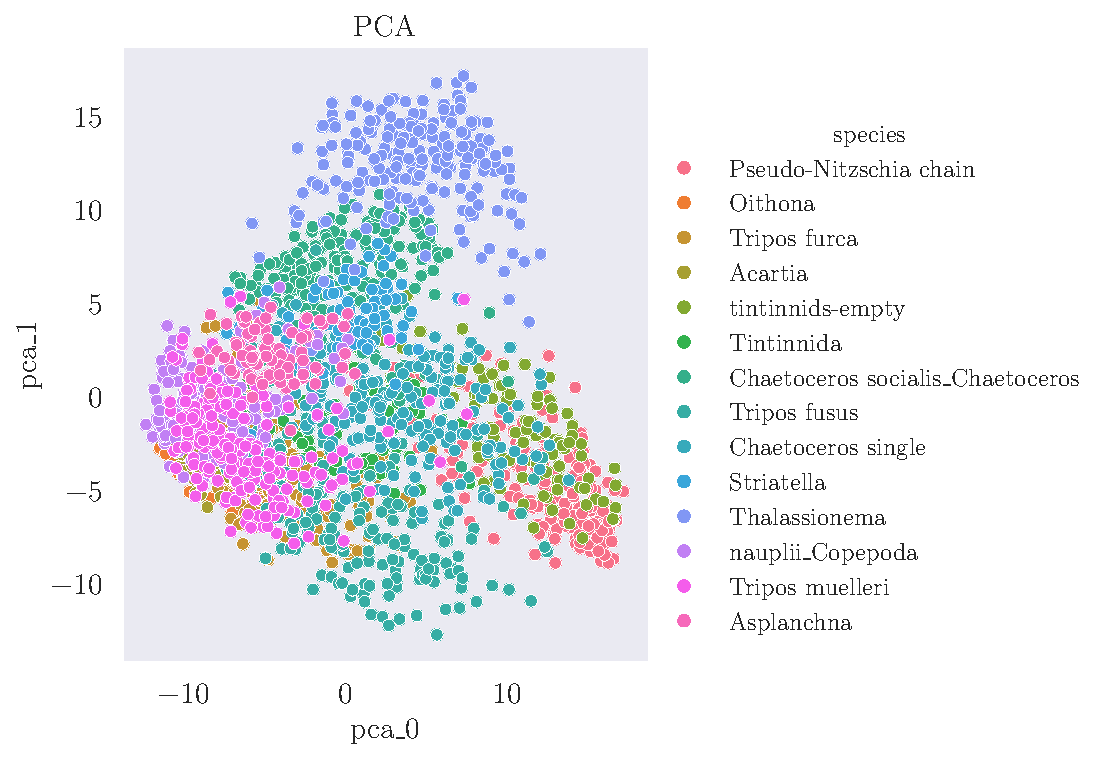
\includegraphics[width=1.1\linewidth]{examples/tests_eb/figs/pca0_pca1.pdf}
    \caption{The two first principal components out of 70 plotted against each other. Already here we can see some weak signs of clusters}
    \label{fig:pca0pca1}
\end{figure}

\begin{figure}[H]
    \centering
    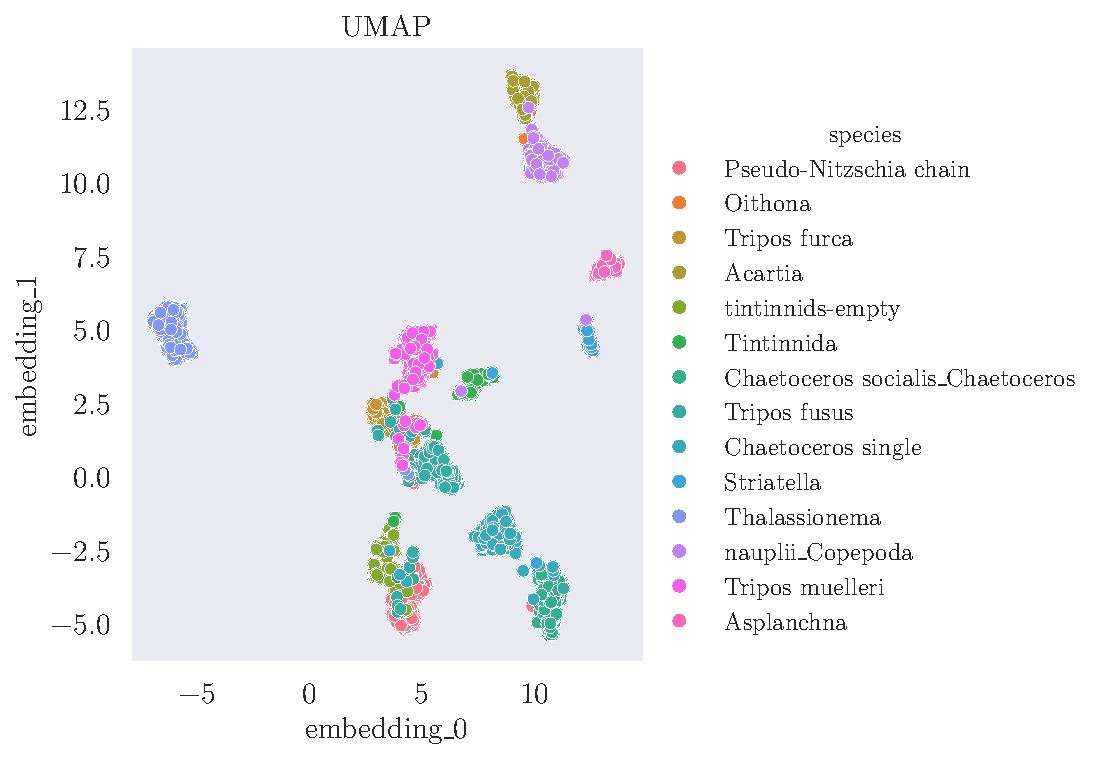
\includegraphics[width=1.1\linewidth]{examples/tests_eb/figs/umap.pdf}
    \caption{A UMAP plot to explore non-linear relations in our data (TODO - read up on UMAP). Here we can clearly see how our extracted features cluster together, yet we still do not have 14 distinct clusters.}
    \label{fig:umap}
\end{figure}

\begin{figure}[H]
    \centering
    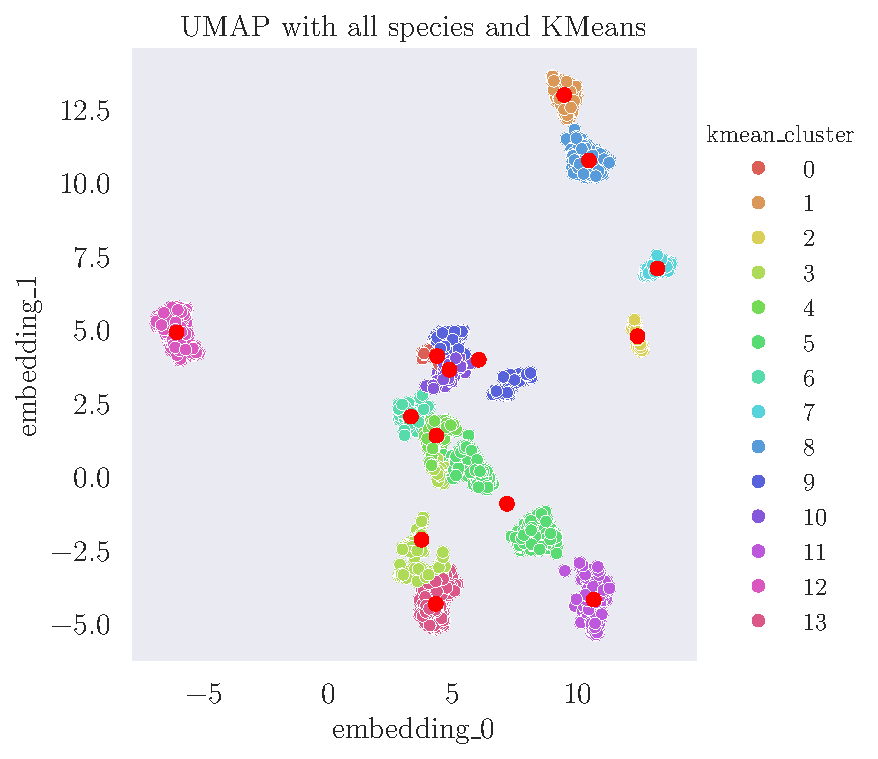
\includegraphics[width=1\linewidth]{latex/figures/kmeans_cluster_umap_on_all_species.pdf}
    \caption{A UMAP with KMeans centroids, which were set to 14 clusters although silhouette coefficients suggested 11. We can clearly see how some centroids are quite close, and arguably even too close for any distinction of the two clusters. We can also see how there appears to be some non-logical centroid placements, as is the case with centroids around 5 (green) and 9 (blue).}
    \label{fig:14-mer-umap}
\end{figure}

\begin{figure}[H]
    \centering
    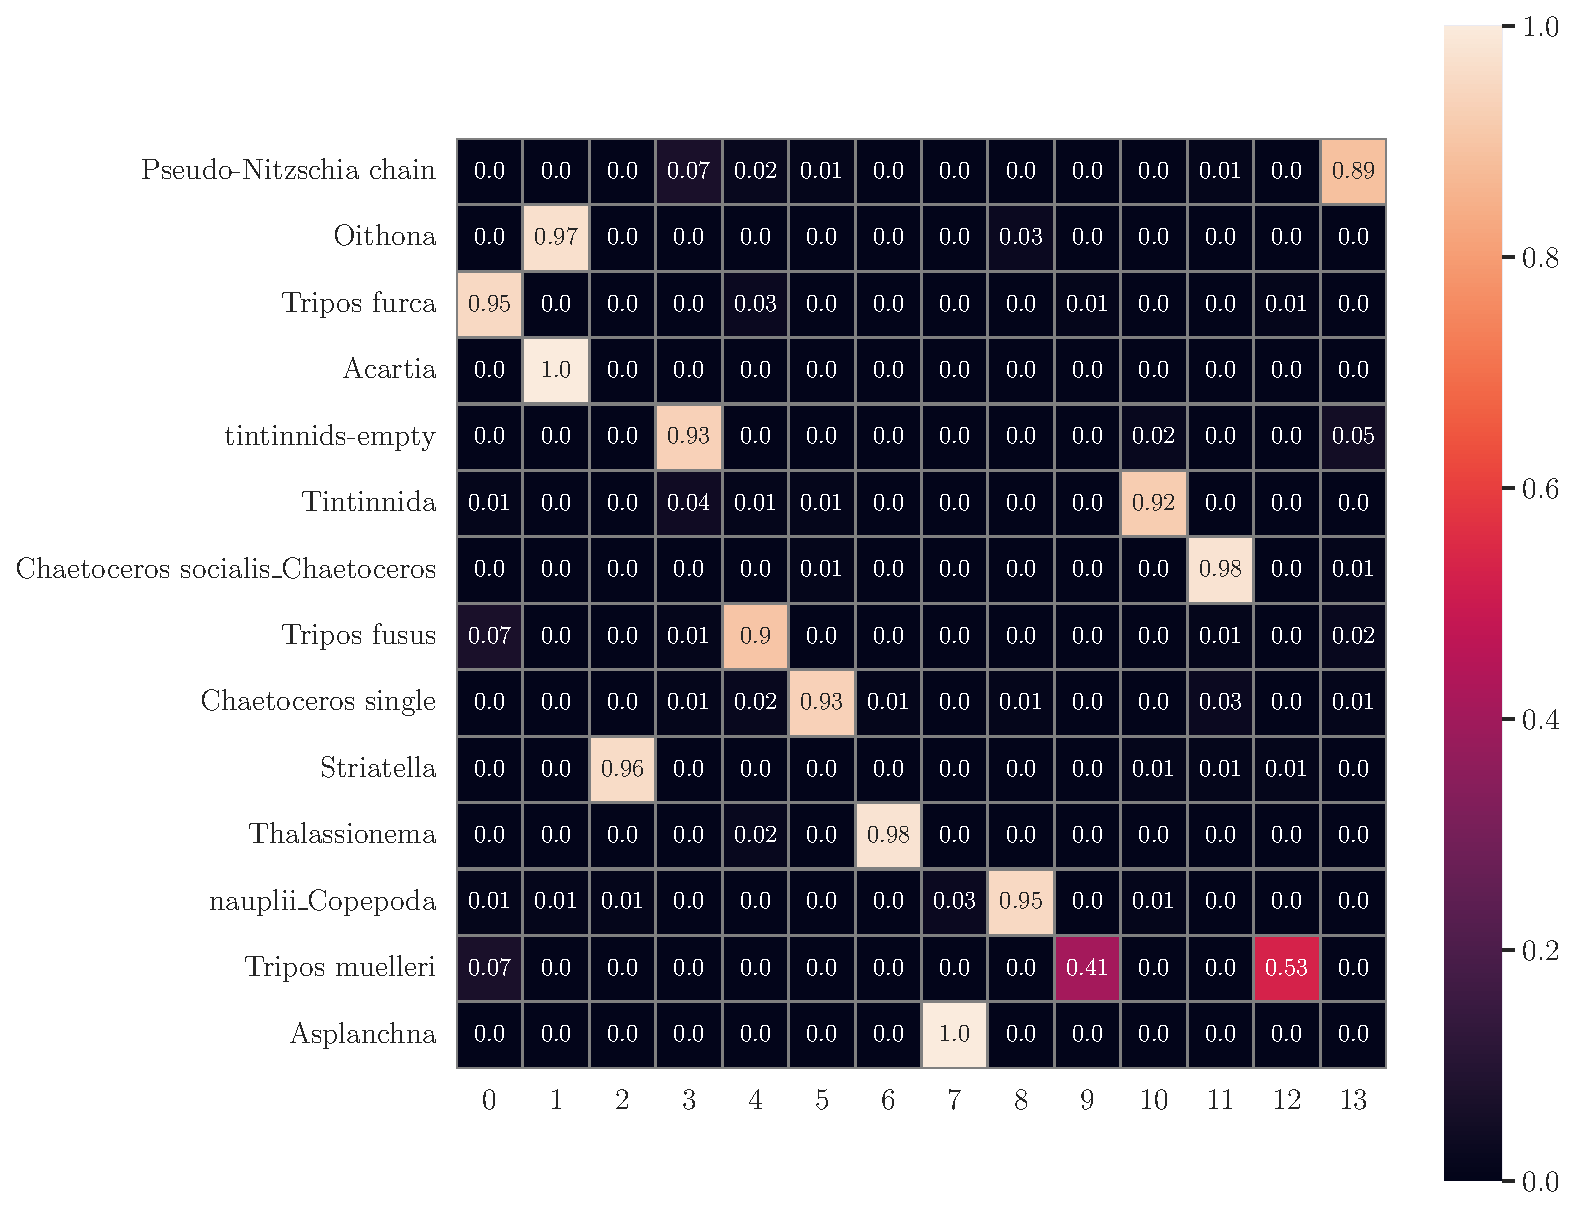
\includegraphics[width=1\linewidth]{latex/figures/dinov2_confmat.pdf}
    \caption{A pseudo-confusion matrix of the unlabeled k-mer centrods and the percentage of species classified withing a k-mer. The total sum of each row adds up to one, so each row presents the distribution of a species within the 14 k-mer clusters. We can see here how \textit{Tripos muelleri} are placed in the dubious 9-mer cluster mentioned in Figure \ref{fig:14-mer-umap}}
    \label{fig:dinov2-confusion}
\end{figure}

\begin{figure}[H]
    \centering
    % Første subfigur
    \begin{subfigure}[b]{0.32\linewidth}
        \centering
        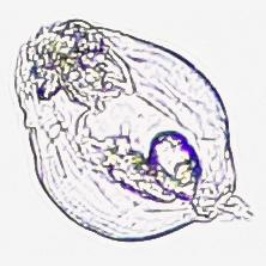
\includegraphics[width=\linewidth]{examples/tests_eb/figs/plankton_examplebatch/asplanktia.png}
        \caption{Species Asplanchna}
        \label{fig:asplanch}
    \end{subfigure}
    % Andre subfigur
    \begin{subfigure}[b]{0.32\linewidth}
        \centering
        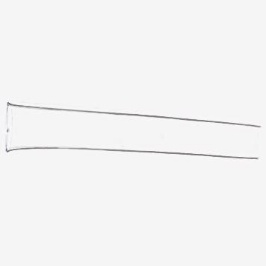
\includegraphics[width=\linewidth]{examples/tests_eb/figs/plankton_examplebatch/empty.jpg}
        \caption{Species Tintinnids-empty}
        \label{fig:empty}
    \end{subfigure}
    % Tredje subfigur
    \begin{subfigure}[b]{0.32\linewidth}
        \centering
        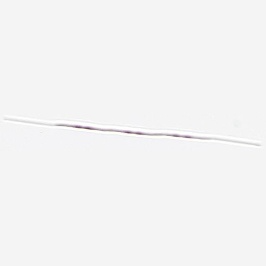
\includegraphics[width=\linewidth]{examples/tests_eb/figs/plankton_examplebatch/pseudo.png}
        \caption{Species Pseudo-Nitzschia}
        \label{fig:pseudo}
    \end{subfigure}
    \caption{In (a), we see an example of a species that has a clear, separate cluster in Figure \ref{fig:umap}. We compare this to (b) and (c), which seemingly cluster together in the same figure.}
    \label{fig:grid}
\end{figure}

Just for fun, we looked into the species that would have been misclusteded if we used KMeans clustering on the two similar species mentioned in Figure \ref{fig:grid}. 

\begin{figure}[H]
    \centering
    \begin{subfigure}[b]{1\linewidth}
        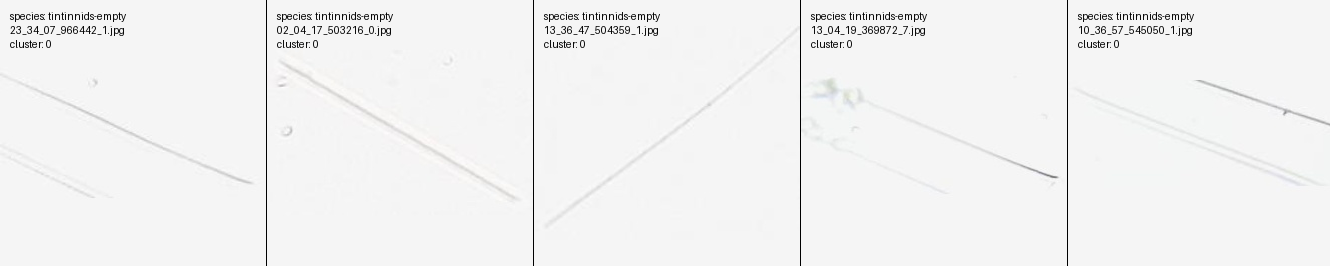
\includegraphics[width=\linewidth]{examples/tests_eb/figs/misclustered_empty.png}
        \caption{Tintinnids-empty that have clustered with Pseudo-Nitzchia chains according to simple K-means clustering of an isolated selection of UMAP embeddings for the two species.}
    \end{subfigure}
    
    \vspace{1em}
    
    \begin{subfigure}[b]{1\linewidth}
        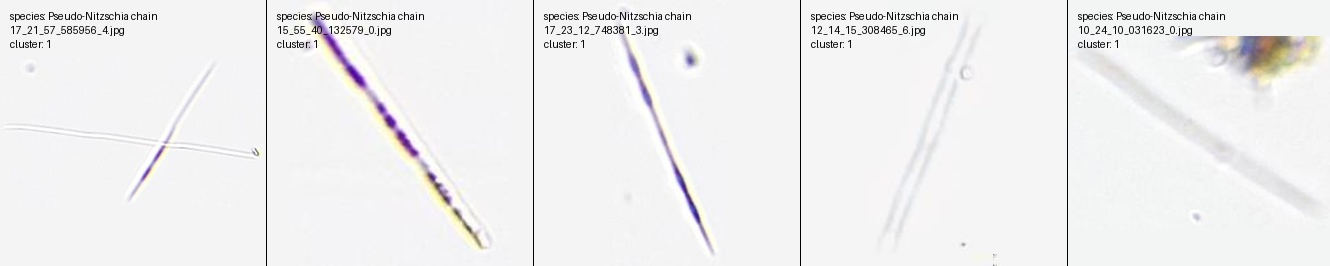
\includegraphics[width=\linewidth]{examples/tests_eb/figs/misclustered_pseudo-nitz.png}
        \caption{Pseudo-Nitzschia chains that have clustered with Tintinnids-empty according to simple K-means clustering of an isolated selection of UMAP embeddings for the two species.}
    \end{subfigure}
    \caption{We compare some of the species that seem to cluster together in Figure \ref{fig:umap} to explore whether the original labels are incorrect or if our DINOv2 fails to discern between the two species. The clustering process demonstrated in Figure \ref{fig:misclustering_process} in our Appendix.}
    \label{fig:misclusters}
\end{figure}


% ==================================================================